\documentclass[11pt]{article}
\usepackage[margin=1in]{geometry}
\usepackage{amsmath, amsfonts}
\usepackage[noend]{algpseudocode}
\usepackage{algorithm}
\usepackage[parfill]{parskip}
\usepackage{enumerate}
\usepackage[shortlabels]{enumitem}
\usepackage{hyperref}
\usepackage[english]{babel}
\usepackage[autostyle]{csquotes}
\usepackage{enumitem}
\usepackage{wrapfig}
\usepackage{tikz}
\usetikzlibrary{decorations.pathreplacing}
\definecolor{color1}{rgb}{0.7, 0.2, 0.2}
\definecolor{color2}{rgb}{0.0, 0.4, 0.0}
\definecolor{color3}{rgb}{0.2, 0.4, 0.7}

%--------------------------------------------------------%


\title{\vspace{-0.5in}Compsci 330 Design and Analysis of Algorithms \\Assignment 6, Spring 2024 Duke University}
\author{Mitch Harrison, Dav King}
\date{Due Date: Thursday, March 7, 2024}

%--------------------------------------------------------%

\begin{document}

\maketitle


%--------------------------------------------------------%

\paragraph{How to Do Homework.} We recommend the following three step process for homework to help you learn and prepare for exams.
\begin{enumerate}
	\item Give yourself ~15-20 minutes per problem to try to solve on your own, without help or external materials, as if you were taking an exam. Try to brainstorm and sketch the algorithm for applied problems. Don't try to type anything yet.
	\item After a break, review your answers. Lookup resources or get help (from peers, office hours, Ed discussion, etc.) about problems you weren't sure about.
	\item Rework the problems, fill in the details, and typeset your final solutions.
\end{enumerate}

\paragraph{Typesetting and Submission.} Your solutions should be typed and submitted as a single pdf on Gradescope. Handwritten solutions or pdf files that cannot be opened will not be graded. \LaTeX \footnote{If you are new to \LaTeX, you can download it for free at \href{https://www.latex-project.org}{latex-project.org} or you can use the popular and free (for a personal account) cloud-editor \href{https://www.overleaf.com}{overleaf.com}. We also recommend \href{https://www.overleaf.com/learn}{overleaf.com/learn} for tutorials and reference.} is preferred but not required. %If you use another editor for your solutions (such as Microsoft Word), you should convert the final document to a pdf, confirm that the symbolic math from the equation editor is properly formatted, and submit the pdf. 
You must mark the locations of your solutions to individual problems on Gradescope as explained in \href{https://help.gradescope.com/article/ccbpppziu9-student-submit-work#submitting_a_pdf}{the documentation}. Any applied problems will request that you submit code separately on Gradescope to be autograded. 

\paragraph{Writing Expectations.} If you are asked to provide an algorithm, you should clearly and unambiguously define every step of the procedure as a combination of precise sentences in plain English or pseudocode. If you are asked to explain your algorithm, its runtime complexity, or argue for its correctness, your written answers should be clear, concise, and should show your work. Do not skip details but do not write paragraphs where a sentence suffices.

\paragraph{Collaboration and Internet.} If you wish, you can work with a single partner (that is, in groups of 2), in which case you should submit a single solution \href{https://help.gradescope.com/article/m5qz2xsnjy-student-add-group-members}{as a group on gradescope}. You can use the internet, but looking up solutions or using large language models is unlikely to help you prepare for exams. See the \href{https://sites.duke.edu/spring24compsci330/policies/}{course policies webpage} for more details.

\paragraph{Grading.} Theory problems will be graded by TAs on an S/U scale (for each sub-problem). Applied problems typically have a separate autograder where you can see your score. The lowest scoring problem is dropped. See the \href{https://sites.duke.edu/spring24compsci330/assignments/}{course assignments webpage} for more details.



%--------------------------------------------------------%


\newpage
\paragraph{Problem 1 (Team Partition).} You are given $n$ players numbered $1, \dots, n$
and a list of $m$ constraints $C = c_1, \dots, c_m$ where each constraint is of the form $(i, j)$ and means that players $i$ and $j$ cannot be placed on the same team. Your goal is to partition the players into two teams $T_A$ and $T_B$ such that every player is assigned to one team and no constraints are violated. Teams do not have to be the same size.

For example, suppose there are $n=4$ players and you have the constraints $(1, 2)$ and $(2, 4)$. Then you could partition the players into teams $T_A = \{1, 4\}$ and $T_B = \{2, 3\}$. However, if you had the additional constraint $(1, 4)$, it becomes impossible to give a valid partition.

Describe a $O(n+m)$ runtime algorithm that either computes and returns a valid partition or returns that none exists. Prove the correctness of the algorithm and analyze its runtime complexity.

You may use DFS, BFS, Dijkstra's algorithm, or the Bellman-Ford algorithm as described in lecture without restating the algorithm or arguing for its correctness. If you modify the algorithm, make sure to be precise about how and explain why any modifications are correct.

\paragraph{Solution}
We will modify \Call{DFS}{} to check to check for constraints while building out
teams. Let $p$ be the id of a player and $t$ be a team, where $t_{A}$ is team
A and $t_{B}$ is team B. Assume that these teams (and the \texttt{valid} 
variable) defined in \Call{teamWrapper}{} are globally available to 
\Call{mdfs}{}.

\begin{algorithm}
\caption{Wrapper function for instantiating global variables}
\begin{algorithmic}[1]
\Procedure{teamWrapper}{$n,m,C$}
    \State $valid \leftarrow True$
    \State $v \leftarrow []$
    \Comment{length-$n$ boolean array for tracking visited players}
    \State $t_{A} \leftarrow \{\}$
    \State $t_{B} \leftarrow \{\}$
    \State \Call{mdfs}{1, "A"}
    \State \Return $valid, t_{A}, t_{B}$
\EndProcedure 
\end{algorithmic}
\end{algorithm}

\begin{algorithm}
\caption{Modified DFS for Question 1}
\begin{algorithmic}[1]
\Procedure{mdfs}{$p,t$}
    \If{$valid = False$}
        \State \Return 
        \Comment{stop exploring this branch}
    \EndIf
    \State $visited[p] \leftarrow True$
    \If{$t = "A"$}
        \State add $p$ to $t_{A}$
    \ElsIf{$t = "B"$}
        \State add $p$ to $t_{B}$
    \EndIf
    \For{all players $j$ not yet explored}
        \If{$(p,j) \in C$ \textbf{and} $j \notin visited$}
        \Comment{if a constraint exists, put on opposite team}
            \If{$t = "A"$}
                \State \Call{mdfs}{$j, "B"$}
            \ElsIf{$t = "B"$}
                \State \Call{mdfs}{$j, "A"$}
            \EndIf
        \ElsIf{$(p,j) \notin C$ and $valid = True$}
        \Comment{no constraint and still valid exploration}
            \State \Call{mdfs}{$j,t$}
            \Comment{assign to same team}
        \EndIf
        \If{\Call{length}{$v$} == $n$}
        \Comment{all players have been visited}
            \If{\Call{size}{$t_{A}$} + \Call{size}{$t_{B}$} = $n$}
            \Comment{all players on teams}
                \State \Return $valid, t_{A}, t_{B}$
            \EndIf
        \EndIf
    \EndFor
\EndProcedure 
\end{algorithmic}
\end{algorithm}

\pagebreak

\paragraph{Proof}
Let $P$ be our set of players, $C$ be our constraints, $V$ be an array that
tracks visited players, and $t_{i}$ be the team that player $i$ resides in. The
$valid$ parameter is \texttt{True} if a branch of exploration is still feasable,
taking constraints into account.

Our \textbf{base case} is when $valid$ is \texttt{False}. In this case, our
current branch of exploration is invalid, and no further exploration occurs.
\textbf{Assume} for a given player $i$ and team $t_{i}$, if $i \in V$, then
$t_{i}$ must be defined and correct (i.e., player has a team and no players
are on two different teams). We will call these assignments "valid."
Additionally, we assume that assigning $i$ to team $t$ does not violate any 
constraints.

During exploration, we always mark newly explored players as visited by setting
$V[i] = True$, meaning that a player cannot be assigned twice. Assigning $p$ to
team $t$ maintains correctness by checking for contraints and ensuring that
the assigned player hasn't been visited. Recursive calls to \Call{mdfs}{}
uphold the IH for neighboring players.

If no valid assignment exists for a branch, $valid$ is set to \texttt{False} to
cease exploration, which is correct behavior. Finally, if all players have
been explored (i.e., $V$ has length $n$), we return the desired effects.

Because the base case is trivially correct, and each inductive step correctly
assigned players to teams given constraints, \Call{mdfs}{} is correct.

\paragraph{Runtime}
This algorithm is a simple alteration to a traditional DFS, with some 
constant-time boolean checks thrown in. Thus, it has the same runtime as
DFS, which is $O(n+m)$, our desired result.

%--------------------------------------------------------%
\newpage
\paragraph{Problem 2 (Probabilistic Routing).} You are routing packets of information along a lossy network. You are given a connected, undirected, weighted graph $G = (V, E)$ with $|V| = n$ and $|E| = m$, where the edge weights are real numbers in $(0, 1)$ corresponding to probabilities. The success probability along a path is the product of the probabilities of its edges.  

For example, the success probability along the path $A, B, C, F$ in the graph diagrammed below is $(1/2)(9/10)(1/4) \approx 11\%$ whereas the success probability along the path $A, D, E, F$ is $(8/10)(9/10)(9/10) \approx 65\%$.

\begin{figure}[!h]
\centering
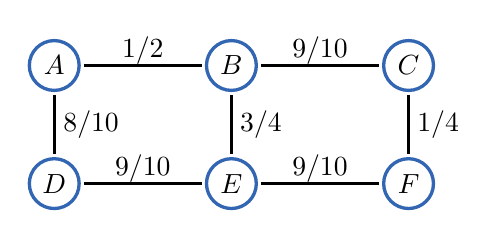
\begin{tikzpicture}[yscale = 0.75, xscale = 0.75]

\draw [very thick, color3] (-3, 1) circle (12pt);
\draw [very thick, color3] (-3, -1) circle (12pt);
\draw [very thick, -] (-2.5, 1) -- (-0.5, 1);
\draw [very thick, -] (-2.5, -1) -- (-0.5, -1);
\draw [very thick, color3] (0, 1) circle (12pt);
\draw [very thick, color3] (0, -1) circle (12pt);
\draw [very thick, -] (0.5, 1) -- (2.5, 1);
\draw [very thick, -] (0, 0.5) -- (0, -0.5);
\draw [very thick, -] (-3, 0.5) -- (-3, -0.5);
\draw [very thick, -] (3, 0.5) -- (3, -0.5);
\draw [very thick, color3] (3, 1) circle (12pt);
\draw [very thick, color3] (3, -1) circle (12pt);
\draw [very thick, -] (0.5, -1) -- (2.5, -1);
\node at (-3, 1) {$A$}; \node at (-3, -1) {$D$};
\node at (0, 1) {$B$}; \node at (0, -1) {$E$};
\node at (3, 1) {$C$}; \node at (3, -1) {$F$};
\node at (-1.5, 1.25) {$1/2$}; \node at (1.5, 1.25) {$9/10$};
\node at (-2.375, 0) {$8/10$}; \node at (0.5, 0) {$3/4$}; \node at (3.5, 0) {$1/4$};
\node at (-1.5, -0.75) {$9/10$}; \node at (1.5, -0.75) {$9/10$};
\end{tikzpicture}
\end{figure}

Describe an algorithm for computing the maximum probability with which a packet can be routed from a source $s$ to a target $t$. Prove that the algorithm is correct and analyze analyze its running time. Make your algorithm as asymptotically efficient as possible.

You may use DFS, BFS, Dijkstra's algorithm, or the Bellman-Ford algorithm as described in lecture without restating the algorithm or arguing for its correctness. If you modify the algorithm, make sure to be precise about how and explain why any modifications are correct.

%--------------------------------------------------------%

\paragraph{Solution}
We will solve this problem using a modified version of Djikstra's algorithm,
but using a priority queue implemented with a max-heap. The heap will prioritize
nodes with the highest probability $p$ of reaching the target. That is, the
inverse of the edge weight. Let $visited$ be an array used to track which nodes
have been traversed, with all values initialized to \texttt{False}. Let $Q$ be
our priority queue, and let $P$ be an array for tracking probabilities. Assume
$P$ and $Q$ to be globally accessable. Also, let $w(u,v)$ be the weight
of an edge from node $u$ to $v$. Let $t$ be our target node, as stated in the
problem.

\begin{algorithm}
\caption{Wrapper procedute for initializing globals}
\begin{algorithmic}[1]
\Procedure{wrapper}{$G, s, t$}
    \State $visited \leftarrow []$
    \Comment{initialize whole array to False}
    \State $Q \leftarrow $ \Call{PriorityQueue}{}
    \State $P \leftarrow []$
    \State add source node $s$ to $Q$
    \State $P[s] \leftarrow 1$
    \State \Call{getRoute}{}
    \State \Return $P[t]$
\EndProcedure 
\end{algorithmic}
\end{algorithm}

\begin{algorithm}
\caption{Modified Dijkstra's algorithm using max-heap priority queue}
\begin{algorithmic}[1]
\Procedure{getRoute}{}
    \While{$Q$ is non-empty}
        \State pop node $u$ from $Q$ with highest $P$.
        \State $visited[u] = True$
        \For{each neighbor $v$ of $u$}
            \State $p_{new} = P[u] * w(u,v)$
            \If{$p_{new} > P[v]$}
                \State $p[v] = p_{new}$
                \State add $v$ to $Q$ with probability $P[v]$
            \EndIf
        \EndFor
    \EndWhile
\EndProcedure 
\end{algorithmic}
\end{algorithm}

\paragraph{Proof}
We initialize $P[s] = 1$ because a packet cannot be lost if it never leaves its
source. This is trivially correct. \textbf{Assume} for all nodes $v$ traversed
before a given node $u$, $P[v]$ correctly represents the maximum probability of
reaching node $v$ from the source node $s$.

Observe that when a node $u$ is dequeued from $Q$, it definitionally has the
highest $P[u]$ value because it is implemented with a max-heap. This means that
the maximum probability path to node $u$ is $P[u]$. Then, for each neighbor of
node $u$ (call these neighbors $v$), we calculate the updated probability by
multiplying the optimal path so far ($P[u]$) by all of the neighbor weights
$w(u,v)$. The maximum probability is taken and assigned to $P[v]$. Since we have
considered all neighbors of our best path so far, and locally choose the best 
path, after we have traversed the whole graph, we find the optimal prbability,
which is at position $P[t]$.

\paragraph{Runtime}
This is a modified version of Dijkstra's algorithm. The subtle distinction is
using a max-heap priority queue and multiplying weights instead of adding them.
Since these changes all involve constant time operations, the runtime is the
same as Dijkstra, which is $O(|E| log(|V|))$.

\newpage
\paragraph{Problem 3 (Useless Edges).} Let  $G=(V, E)$ be a directed graph, not necessarily acyclic, with  $|V|=n$, $|E|=m$ and with positive edge weights $w(u, v)$ for every $u \rightarrow v \in E$. For given vertices $s$ and $t$, note that there may be multiple shortest paths from $s$ to $t$. For example, there are three distinct shortest paths from $A$ to $F$ in the following figure (edges of these paths drawn as solid lines).

\begin{figure}[!h]
\centering
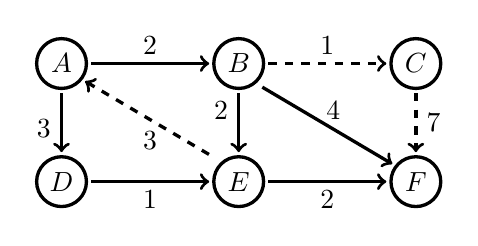
\begin{tikzpicture}[yscale = 0.75, xscale = 0.75]
\draw [very thick] (-3, 1) circle (12pt);
\draw [very thick] (-3, -1) circle (12pt);
\draw [very thick] (0, 1) circle (12pt);
\draw [very thick] (0, -1) circle (12pt);
\draw [very thick] (3, 1) circle (12pt);
\draw [very thick] (3, -1) circle (12pt);
\node at (-3, 1) {$A$}; \node at (-3, -1) {$D$};
\node at (0, 1) {$B$}; \node at (0, -1) {$E$};
\node at (3, 1) {$C$}; \node at (3, -1) {$F$};
\draw [very thick, ->] (-2.5, 1) -- (-0.5, 1); \node at (-1.5, 1.3) {$2$};
\draw [very thick, dashed, <-] (-2.6, 0.7) -- (-0.4, -0.6); \node at (-1.5, -0.3) {$3$};
\draw [very thick, ->] (-2.5, -1) -- (-0.5, -1); \node at (-1.5, -1.3) {$1$};
\draw [very thick, dashed, ->] (0.5, 1) -- (2.5, 1); \node at (1.5, 1.3) {$1$};
\draw [very thick, ->] (0, 0.5) -- (0, -0.5); \node at (-0.3, 0.2) {$2$};
\draw [very thick, ->] (0.4, 0.6) -- (2.6, -0.7); \node at (1.6, 0.2) {$4$};
\draw [very thick, ->] (-3, 0.5) -- (-3, -0.5); \node at (-3.3, -0.1) {$3$};
\draw [very thick, dashed, ->] (3, 0.5) -- (3, -0.5); \node at (3.3, 0.0) {$7$};
\draw [very thick, <-] (2.5, -1) -- (0.5, -1); \node at (1.5, -1.3) {$2$};
\end{tikzpicture}
\end{figure}

Describe an algorithm that, given vertices $s$ and $t$, returns the number of edges in the graph that are \textit{not} included in \textit{any} shortest paths from $s$ to $t$. In the example graph above with $s=A$ and $t=F$ there are three such edges (drawn in dashed lines). Prove that the algorithm is correct and analyze analyze its running time. Make your algorithm as asymptotically efficient as possible.

You may use DFS, BFS, Dijkstra's algorithm, or the Bellman-Ford algorithm as described in lecture without restating the algorithm or arguing for its correctness. If you modify the algorithm, make sure to be precise about how and explain why any modifications are correct.

\paragraph{Solution 3 (Algorithm)}

\begin{algorithmic}[1]
    \Procedure{uselessEdges}{s, t, G}
        \State Run Dijkstra's algorithm to get the distance from $s$ to every $V \in G$
        \State Run Dijkstra's algorithm on $G^r$ to get the distance from every $V \in G$ to $t$
        \State $n = 0$
        \For{$E \in G$}
            \State $u$ = source of $E$
            \State $v$ = destination of $E$
            \State $x$ = dist$(s, u)$ + $w(u, v)$ + dist$(v, t)$ \Comment{stored from Dijkstra's}
            \If{$x >$ dist$(s, t)$}
                \State n++
            \EndIf
        \EndFor
        \State \Return n
    \EndProcedure
\end{algorithmic}

As a note: When running Dijkstra's algorithm on $G$ or $G^r$ (the reverse graph), the distances from $s$ to all nodes and from all nodes to $t$ (i.e., from $t$ to all nodes in the reverse graph) need to be stored. This can be done in a simple array, which has constant lookup.

\paragraph{Solution 3 (Proof)}

\begin{itemize}
    \item \textbf{Given:} Dijkstra's algorithm correctly records the unique length of the shortest path from $s$ to $t$. While it may not return all shortest paths, this is irrelevant.
    \item \textbf{Given:} Dijkstra's algorithm also correctly records the shortest path from $s$ to all $u \in V$ and from all $v \in V$ to $t$.
    \item \textbf{Given:} there can be only one edge from $u$ to $v$.
    \item \textbf{Assume} $(u, v)$ is on the shortest path dist$(s, t)$; i.e., $x =$ dist$(s, t)$.
    \item \textbf{Let} $y =$ dist$(s, t)$ - dist$(s, u)$ - dist$(v, t)$.
    \item \textbf{If} $y = w(u, v)$, then $(u, v)$ is indeed on the shortest path, and $x =$ dist$(s, t)$ correctly. This is because dist$(s, u)$ is already the shortest path from $s$ to $u$ and dist$(v, t)$ is already the shortest path from $v$ to $t$, so the only way to satisfy $x =$ dist$(s, t)$ is if $(u, v)$ is contained on this shortest path.
    \item \textbf{If} $y > w(u, v)$ then the shortest path cannot include $(u, v)$, because in order to satisfy $x =$ dist$(u, v)$ we would require either dist$(s, u)$ or dist$(v, t)$ to indeed \textit{not} be their respective shortest paths, a \textbf{contradiction}.
    \item \textbf{Therefore:} by adding up all such edges, we return the total number of edges that are not contained on any shortest path (i.e., the edges for whom the shortest path containing $(u, v)$ is longer than the shortest path dist$(s, t))$.
\end{itemize}

\paragraph{Solution 3 (Runtime)}

We know that running Dijkstra's algorithm comes with a runtime $O((n + m)\text{log}(n))$; running this twice does not change that runtime. Then, we simply iterate over all $m$ edges. Since we have stored the distances from $s$ to all vertices and from all vertices to $t$ in arrays with constant time lookup, and since looking up the edge weights is also a constant time operation, all we do in this loop is constant time; thus, the loop runs in $O(m)$ time. Since this $O(m)$ runtime (run sequentially after the Dijkstra's calls) is dominated by the runtime of Dijkstra's algorithm, we report that the runtime of this full algorithm is $O((n + m)\text{log}(n))$.

%--------------------------------------------------------%

\newpage
\paragraph{Problem 4 (Applied).}  Your are working at an investment firm and are given the task to build an auto-detector for arbitrage ("risk-free" profit) opportunity from the currency exchange market. Given a list of exchange rates, your detector should tell you if you can make profit and a currency exchange "path" you can follow to make profit (if such opportunity exists).

Suppose the current exchange rate is:
\begin{align*}
    USD\xrightarrow{130}JPY\hspace{3em}
    JPY\xrightarrow{0.006}GBP\hspace{3em}
    GBP\xrightarrow{1.3}USD
\end{align*}
Then starting with 1 USD, you can convert it along USD-JPY-GBP-USD and get $130\times 0.006\times 1.3=1.014$ USD, which is more that what you have initially. We call such path an \textit{arbitrage path}, since we can earn guaranteed profit from the trades. 

The exchange rates are represented by $(i,j,w_{ij})$ tuples, where $i$, $j$ are integers representing types of currencies and $w_{ij}$ is the exchange rate (1 unit of currency $i$ exchanges to $w_{ij}$ units of currency $j$). Let $V$ be the set of currencies and $E$ the set of exchange rate tuples. You want to find a path that starts with currency $v_i$, goes through $v_{i+1}$, $v_{i+2}$,$\dots$ $v_{i+k}$ and ends at $v_i$ so that the products of their corresponding rates are greater than 1 ($w_{i,i+1}w_{i+1,i+2}\dots w_{i+k,i}> 1$) for some $k\leq|V|$. 


\textbf{You will need to design and implement an algorithm that efficiently determines an arbitrage path, if it exists.} Your solution will need to have an empirical runtime that is within constant factors of an reference solution with  $O(|V||E|)$ worst case runtime. If there are multiple arbitrage paths, you algorithm only needs to return one and the choice of starting currency doesn't matter. Also note that the existence of $(i,j, w_{ij})$ doesn't imply the existence of $(j,i, 1/w_{ij})$.

\textit{Hint: How could you modify the exchange rates to use an existing algorithm? } 

Language-specific details follow. You can use whichever of Python or Java you prefer. You will receive automatic feedback when submitting, and you can resubmit as many times as you like up to the deadline. \textbf{NOTE:} Unlike the theory problems, the applied problem grade \textbf{is the raw score shown on Gradescope}. See the \href{https://sites.duke.edu/spring24compsci330/assignments/}{course assignments webpage} for more details. 

\begin{itemize}
	\item \textbf{Python.} You should submit a file called \texttt{arbitrage.py} to the Gradescope item "Assignment 3 - Applied (Python)." The file should define (at least) a top level function \texttt{arbitrage} that takes in a list of tuples \texttt{(i:int, j:int, w:float)} and returns:
	\begin{itemize}
	    \item If an arbitrage path exists: \texttt{[\ ]} - a list of integers that are ordered to form an arbitrage path
	    \item Otherwise: \texttt{None}
	\end{itemize}
	For example, your algorithm should return \texttt{[1,2,3,1]}, if we take USD as currency 1, JPY as currency 2 and GBP as currency 3,
	

\item \textbf{Java.} You should submit a file called \texttt{Arbitrage.java} to the Gradescope item "Assignment 3 - Applied (Java)." The file should define (at least) a top level function \texttt{arbitrage} that takes in a 2D array of currencies and an array of weights where the conversion rate from \texttt{currencies[i][0]} to \texttt{currencies[i][1]} is \texttt{weight[i]}. The method header should be as follows: 
    \begin{itemize}
        \item \texttt{public List<Integer> arbitrage(int[][] currencies, double[] weights);}
    \end{itemize}
    As shown the header, the output should be a list of integers, which is the arbitrage path, if there is one. If there is no path, return \texttt{null}. For example, your algorithm should return \texttt{[1,2,3,1]} if we take USD as currency 1, JPY as currency 2, and GBP as currency 3.
\end{itemize}

\end{document}
